\documentclass[11pt]{article}\usepackage[]{graphicx}\usepackage[]{color}
%% maxwidth is the original width if it is less than linewidth
%% otherwise use linewidth (to make sure the graphics do not exceed the margin)
\makeatletter
\def\maxwidth{ %
  \ifdim\Gin@nat@width>\linewidth
    \linewidth
  \else
    \Gin@nat@width
  \fi
}
\makeatother

\definecolor{fgcolor}{rgb}{0.345, 0.345, 0.345}
\newcommand{\hlnum}[1]{\textcolor[rgb]{0.686,0.059,0.569}{#1}}%
\newcommand{\hlstr}[1]{\textcolor[rgb]{0.192,0.494,0.8}{#1}}%
\newcommand{\hlcom}[1]{\textcolor[rgb]{0.678,0.584,0.686}{\textit{#1}}}%
\newcommand{\hlopt}[1]{\textcolor[rgb]{0,0,0}{#1}}%
\newcommand{\hlstd}[1]{\textcolor[rgb]{0.345,0.345,0.345}{#1}}%
\newcommand{\hlkwa}[1]{\textcolor[rgb]{0.161,0.373,0.58}{\textbf{#1}}}%
\newcommand{\hlkwb}[1]{\textcolor[rgb]{0.69,0.353,0.396}{#1}}%
\newcommand{\hlkwc}[1]{\textcolor[rgb]{0.333,0.667,0.333}{#1}}%
\newcommand{\hlkwd}[1]{\textcolor[rgb]{0.737,0.353,0.396}{\textbf{#1}}}%

\usepackage{framed}
\makeatletter
\newenvironment{kframe}{%
 \def\at@end@of@kframe{}%
 \ifinner\ifhmode%
  \def\at@end@of@kframe{\end{minipage}}%
  \begin{minipage}{\columnwidth}%
 \fi\fi%
 \def\FrameCommand##1{\hskip\@totalleftmargin \hskip-\fboxsep
 \colorbox{shadecolor}{##1}\hskip-\fboxsep
     % There is no \\@totalrightmargin, so:
     \hskip-\linewidth \hskip-\@totalleftmargin \hskip\columnwidth}%
 \MakeFramed {\advance\hsize-\width
   \@totalleftmargin\z@ \linewidth\hsize
   \@setminipage}}%
 {\par\unskip\endMakeFramed%
 \at@end@of@kframe}
\makeatother

\definecolor{shadecolor}{rgb}{.97, .97, .97}
\definecolor{messagecolor}{rgb}{0, 0, 0}
\definecolor{warningcolor}{rgb}{1, 0, 1}
\definecolor{errorcolor}{rgb}{1, 0, 0}
\newenvironment{knitrout}{}{} % an empty environment to be redefined in TeX

\usepackage{alltt}    
%\usepackage[latin1]{inputenc}
\usepackage[parfill]{parskip} % Activate to begin paragraphs with an empty line rather than an indent
\usepackage{amsmath,amsthm,amssymb,bbm} %math stuff
\usepackage{ctable}
\usepackage{placeins} % FloatBarrier
\usepackage{fancyhdr}
\usepackage{lastpage}
\usepackage{float}    % for fig.pos='H'
\usepackage{rotfloat} % for sidewaysfigure
%\usepackage{subfig}   % for subfigure
\usepackage{subcaption}  % an alternative package for sub figures
\newcommand{\subfloat}[2][need a sub-caption]{\subcaptionbox{#1}{#2}}
\usepackage{comment}
\usepackage[round]{natbib}   % omit 'round' option if you prefer square brackets
\bibliographystyle{plainnat}
\usepackage{setspace} %Spacing
\usepackage{graphicx,graphics}
\usepackage{booktabs,tabularx}
\usepackage{enumerate}
\usepackage{makecell}
\usepackage{xfrac}
\usepackage{color, colortbl, xcolor}
\usepackage{booktabs,dcolumn} % for use with texreg in R
\usepackage[pagebackref=true,bookmarks]{hyperref}
\hypersetup{
    unicode=false,          
    pdftoolbar=true,        
    pdfmenubar=true,        
    pdffitwindow=false,     % window fit to page when opened
    pdfstartview={FitH},    % fits the width of the page to the window
    pdftitle={004-Figures},    % title
    pdfauthor={SRB},     % author
    pdfsubject={Subject},   % subject of the document
    pdfcreator={SRB},   % creator of the document
    pdfproducer={SRB}, % producer of the document
    pdfkeywords={}, % list of keywords
    pdfnewwindow=true,      % links in new window
    colorlinks=true,       % false: boxed links; true: colored links
    linkcolor=red,          % color of internal links (change box color with linkbordercolor)
    citecolor=blue,        % color of links to bibliography
    filecolor=black,      % color of file links
    urlcolor=cyan           % color of external links
}
\IfFileExists{upquote.sty}{\usepackage{upquote}}{}
\begin{document}
%\pagestyle{fancy}

\title{Prerequisite Skill Structures in ASSISTments}
\author{Michel Desmarais \and Sameer Bhatnagar}
\date{\today}
\maketitle






\begin{abstract}
At the 2015 Artificial Intelligence in Education conference, Seth Adjei and Neil Heffernan presented their work on scrutinizing expert-defined prerequisite skill graphs. Using randomized controlled trials in PLACEments, the computer-adaptive-testing feature in the ASSISTments learning environment, they were able to identify some prerequisite skill arcs that were not supported by data.\\
This proposal outlines two alternative techniques that could be used to achieve the goal. We will start with a basic introduction to Partial Order Knowledge Structures (POKS), then try to mathematically formalize what a prerequisite skill might mean in this framework. The first proposed technique will be graph based, while the second will be built on interpreting probabilities during POKS structural learning.
\end{abstract}

\section{POKS}
Partial Order Knowledge Structures (POKS) determine which items in a test are prerequisite to others. POKS are derived from the theory of Knowledge Spaces, where such prerequisite relationships are written as $A \to B $, which means if a student got item A correct, they likely will get item B also correct; said differently, item B is a prerequisite of item A.

\subsection{Working Example}
Let us look at a classical dataset from Tatsuoka, which is well studied in de la Torre. 
\begin{knitrout}
\definecolor{shadecolor}{rgb}{0.969, 0.969, 0.969}\color{fgcolor}\begin{kframe}
\begin{verbatim}
## 'data.frame':	536 obs. of  11 variables:
##  $ H01: int  1 1 1 1 1 0 0 1 0 0 ...
##  $ H02: int  1 1 1 0 0 0 0 0 0 0 ...
##  $ H03: int  0 1 0 0 0 1 1 0 1 1 ...
##  $ H04: int  1 1 0 1 0 0 0 0 0 0 ...
##  $ H05: int  1 1 0 1 0 0 0 0 0 0 ...
##  $ H06: int  1 1 0 1 1 0 0 0 1 1 ...
##  $ H08: int  1 1 1 0 0 0 0 0 0 0 ...
##  $ H09: int  1 1 1 1 0 0 0 0 0 0 ...
##  $ H10: int  0 1 0 0 0 0 0 0 0 0 ...
##  $ H11: int  1 1 0 1 0 0 0 0 0 0 ...
##  $ H13: int  1 1 0 1 0 0 0 0 0 0 ...
\end{verbatim}
\end{kframe}
\end{knitrout}

If we run the POKS code on this data, we get the following adjacency matrix.\\
% latex table generated in R 3.2.0 by xtable 1.7-4 package
% Fri Jul 24 23:59:50 2015
\begin{tabular}{rrrrrrrrrrrr}
  \hline
 & 1 & 2 & 3 & 4 & 5 & 6 & 7 & 8 & 9 & 10 & 11 \\ 
  \hline
1 & 0 & 0 & 0 & 0 & 0 & 0 & 0 & 0 & 0 & 0 & 0 \\ 
  2 & 1 & 0 & 1 & 0 & 1 & 1 & 1 & 1 & 0 & 0 & 0 \\ 
  3 & 0 & 0 & 0 & 0 & 0 & 0 & 0 & 0 & 0 & 0 & 0 \\ 
  4 & 1 & 0 & 1 & 0 & 1 & 1 & 1 & 1 & 1 & 1 & 1 \\ 
  5 & 1 & 0 & 0 & 0 & 0 & 1 & 0 & 1 & 1 & 1 & 0 \\ 
  6 & 0 & 0 & 0 & 0 & 0 & 0 & 0 & 0 & 0 & 0 & 0 \\ 
  7 & 1 & 0 & 0 & 0 & 0 & 1 & 0 & 1 & 0 & 0 & 0 \\ 
  8 & 0 & 0 & 0 & 0 & 0 & 0 & 0 & 0 & 0 & 0 & 0 \\ 
  9 & 1 & 0 & 0 & 0 & 1 & 1 & 1 & 1 & 0 & 1 & 1 \\ 
  10 & 0 & 0 & 0 & 0 & 1 & 1 & 0 & 1 & 0 & 0 & 0 \\ 
  11 & 1 & 0 & 0 & 1 & 1 & 1 & 1 & 1 & 1 & 1 & 0 \\ 
   \hline
\end{tabular}

This structure can be visualized as follows:\\
\begin{knitrout}
\definecolor{shadecolor}{rgb}{0.969, 0.969, 0.969}\color{fgcolor}

{\centering 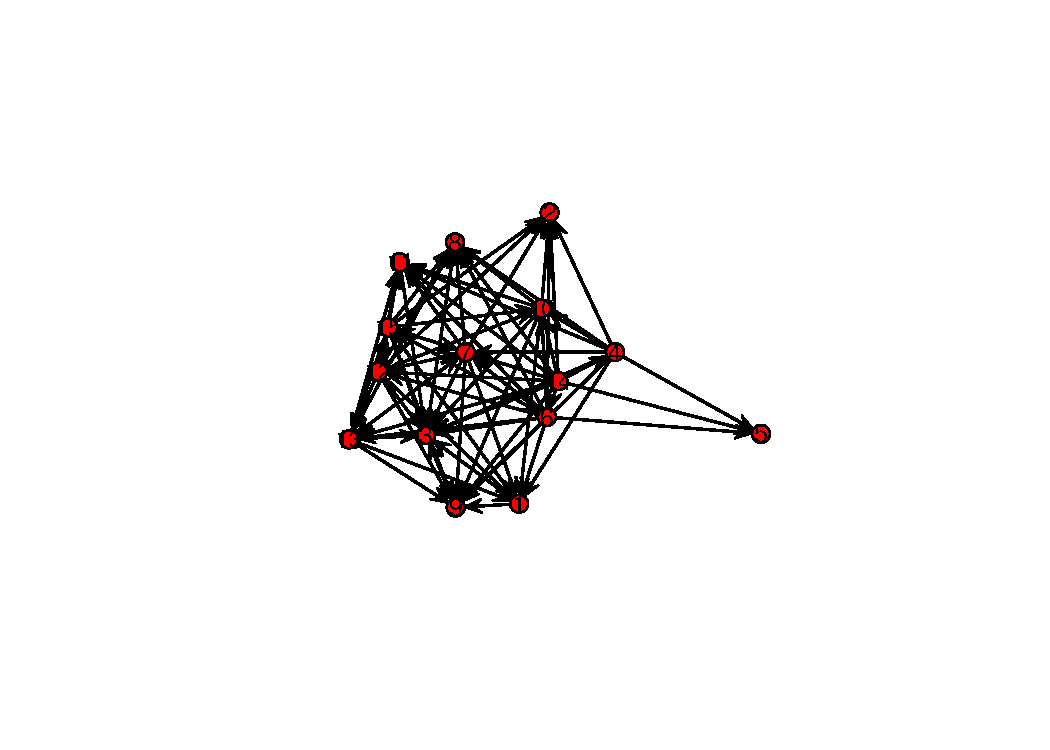
\includegraphics[width=\maxwidth]{figure/poks-graph-1} 

}



\end{knitrout}

What stands out is item three, which has no prerequisites (no edges leaving node 3). Let us use this as a place to work out some numbers to demonstrate how the POKS structure is induced. We see that mastery of item 2 implies mastery of item 3 from the table and the graph. Let us check the contingency table for these two items.\\

\begin{knitrout}
\definecolor{shadecolor}{rgb}{0.969, 0.969, 0.969}\color{fgcolor}\begin{kframe}
\begin{verbatim}
##      item3
## item2   0   1
##     0 149 173
##     1  40 174
\end{verbatim}
\end{kframe}
\end{knitrout}
Now we can calculate $P(item2|item3)$ which should be greater than some threshold, as should $P(\neg item3|\neg item2)$.
We must also ensure that the distributions over the two items are actually interacting with one another using a chi-square test.\\
\begin{knitrout}
\definecolor{shadecolor}{rgb}{0.969, 0.969, 0.969}\color{fgcolor}\begin{kframe}
\begin{verbatim}
## 
## 	Pearson's Chi-squared test with Yates' continuity
## 	correction
## 
## data:  item2 and item3
## X-squared = 40, df = 1, p-value = 1e-10
\end{verbatim}
\end{kframe}
\end{knitrout}

\section{Prerequisite Skills}
It is important to recognize that to go from item-item structures, to skill-skill structure, we need an item-skill mapping. This has been coined the Q-matrix, where each item may require one or more skills. Here is an example of a expert defined q-matrix from our dataset:\\

% latex table generated in R 3.2.0 by xtable 1.7-4 package
% Fri Jul 24 23:59:50 2015
\begin{table}[ht]
\centering
\begin{tabular}{rrrr}
  \hline
 & QH1 & QH2 & QH3 \\ 
  \hline
H01 & 1 & 1 & 0 \\ 
  H02 & 1 & 0 & 1 \\ 
  H03 & 1 & 0 & 1 \\ 
  H04 & 1 & 0 & 0 \\ 
  H05 & 1 & 1 & 0 \\ 
  H06 & 1 & 1 & 0 \\ 
  H08 & 1 & 0 & 1 \\ 
  H09 & 1 & 0 & 1 \\ 
  H10 & 1 & 0 & 0 \\ 
  H11 & 1 & 0 & 0 \\ 
  H13 & 1 & 1 & 0 \\ 
   \hline
\end{tabular}
\end{table}



\section{Deriving Prequisite skills - proposal 1}

\section{Deriving Prequisite skills - proposal 2}
if an item is succeeded, then all the skills involved should be considered succeeded.  If it is failed, then we need to determine how confident we are that skills involved are not mastered. And with the accumulated numbers, we simply build the POKS structure over skills!


\end{document}
